\documentclass[pdftex,a4paper,12pt,twoside,titlepage,italian,openright]{article}
\usepackage[italian]{babel}
\usepackage[utf8]{inputenc}
\usepackage{fancyhdr,graphicx}
\usepackage[hmargin=2cm,vmargin=2cm,a4paper]{geometry}
\usepackage{hyperref}
\usepackage{xcolor}
\pagestyle{fancy}
\lhead{\scshape Curriculum Vitae}
\rhead{\itshape Mauro Donadeo}
\rfoot{\footnotesize pag. \thepage}
\cfoot{}
\lfoot{{\footnotesize Update to: }\today}
\renewcommand{\headrulewidth}{.5pt}
\renewcommand{\footrulewidth}{.5pt}
%\renewcommand{\LettrineFontHook}{\color[gray]{0.5}}
\renewcommand*\familydefault{\sfdefault}
\renewcommand*\labelitemi{$\textcolor{black!30}{\bullet}$}
%\definecolor{listings-comment-color}{RGB}{20,0,0}

\begin{document}
\vspace*{.2cm}
\begin{center}
\rule{.8 \textwidth}{1pt}\\[5pt]
\begin{minipage}{.55\textwidth}
	\LARGE\textbf{Mauro Donadeo}\\[20pt]
	\footnotesize Via Isonzo 136/7 \\ 
	35143 - Padova (PD)\\
	email: \texttt{mauro.donadeo@gmail.com}\\
	\footnotesize n. Tel: +393467846243\\
	\footnotesize Nationality: Italian\\
%	\footnotesize Stato civile: Celibe\\
\end{minipage}
\begin{minipage}{.25\textwidth}
	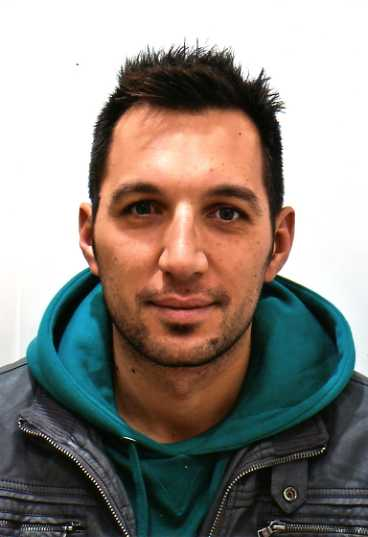
\includegraphics[width=\textwidth]{io.jpg}
\end{minipage}\\[5pt]
\rule{.8 \textwidth}{1pt}
\end{center}
\section*{Actual position:}
 	Worker with University of Padua for develop a system of gesture recognition based on Microsoft Kinect.
\section*{Istruzione}
\begin{itemize}
	\item Master Degree in Computer Engineering (Univeristy of Padua, October 2011).
	Thesis: {\itshape 3D Realtime videoconferencing system based on Microsoft Kinect sensor: design and implementation }
	\item Bachelor Degree in Computer Engineering 
	(University of Padua, April 2008). Thesis:
	{\itshape Realizzazione di un simulatore elementare del sistema robotico Lego Nxt
	in Java}
	\item Diploma Capo-tecnico Informatico (I.T.I.S. A. Meucci di Casarano (LE), 2004)
\end{itemize}
\section*{Esperienze Professionali}
\begin{itemize}
	\item Assistente informatico presso l'ufficio certificazione offerta didattica - SID.
	Presso: Università degli Studi di Padova
	\begin{itemize}
		\item Dal 01-09-2008 al 31-09-2009 
		\item Bonifica dati della base dati dell'Università, area didattica, prendendo come 
		modello i dati provenienti dal ministero.
		\item Creazione di una piccola applicazione web per il controllo delle attività didattiche
		per la generazione del \textit{diploma supplement}.
	\end{itemize}
	\item Assistente informatico presso l'Ufficio Tecnico e Coordinamento Reti. Presso:
	Regione del Veneto
	\begin{itemize}
		\item Dal Dicembre 2007 al Agosto 2008
		\item Progettazione e creazione del portale {\texttt overnetwork.it} basato sul {\textit cms Joomla}
		ed in particolare: creazione di un sistema di \textit{trouble ticketing} con conseguente 
		invio di notifiche tramite mail. Creazione di un nuovo sistema di \textit{profiling}
		degli utenti differente da quello previsto dalla piattaforma Joomla
	\end{itemize}
	\item Portalettere per vari periodi presso i comuni di Cittadella (PD) e Campodarsego (PD).
\end{itemize}
\section*{Conoscenze informatiche:}
\begin{itemize}
	\item \textbf{S.O.:} Gnu/Linux, principalmente, Debian \& Acrhlinux conoscenza 
	che va dall'installazione alla configurazione. Conoscenza anche dei vari 
	sistemi operativi Microsoft.
	\item \textbf{Programmazione: } Esperienze di programmazione con 
	Java, C/C++ (anche con Microsoft Visual Studio 2010),
	esperienze di programmazione web con: php, mySql. 
	\item \textbf{Altro: }\LaTeX, OpenGL, vim, Matlab, pacchetto Office,
	alcune esperienze lavorative con Photoshop e Flash, DirectX10, OpenNI,
	NXC.
\end{itemize}
\section*{Conoscenze linguistiche:}
\begin{itemize}
	\item \textbf{Italiano:} madrelingua;
	\item \textbf{Inglese:} buona conoscenza nella lettura, sufficiente nel parlarlo ed 
	ascoltarlo.
	\item \textbf{Spagnolo:} ottima conoscenza sia scritta che parlata acquisita in un anno
	di Erasmus a Barcellona nel 2009/2010.
\end{itemize}
\section*{Interessi personali: }
\begin{itemize}
	\item Informatica in generale, editing video e immagini
	\item Sport: pratico nuoto e bicicletta, saltuariamente gioco a calcetto;
	\item Libri possibilmente in spagnolo per mantenere la conoscenza della lingua.
\end{itemize}
\vfill
Ai sensi del D. Lgs n. 196/2003 autorizzo al trattamento dei miei dati personali.
\vspace{1cm}
\end{document}
